% Format teze zasnovan je na paketu memoir
% http://tug.ctan.org/macros/latex/contrib/memoir/memman.pdf ili
% http://texdoc.net/texmf-dist/doc/latex/memoir/memman.pdf
% 
% Prilikom zadavanja klase memoir, navedenim opcijama se podešava 
% veličina slova (12pt) i jednostrano štampanje (oneside).
% Ove parametre možete menjati samo ako pravite nezvanične verzije
% mastera za privatnu upotrebu (na primer, u b5 varijanti ima smisla 
% smanjiti 
\documentclass[12pt,oneside]{memoir}
\newcommand\tab[1][0.5cm]{\hspace*{#1}} 
% Paket koji definiše sve specifičnosti master rada Matematičkog fakulteta
\usepackage[latinica,biblatex]{matfmaster} 
\usepackage{verbatim}
\usepackage{url}
\newtheorem{primer}{Primer}

\usepackage[latinica]{pangrami}
\usepackage{listings}
\usepackage{color}
 
\definecolor{codegreen}{rgb}{0,0.6,0}
\definecolor{codegray}{rgb}{0.5,0.5,0.5}
\definecolor{codepurple}{rgb}{0.58,0,0.82}
\definecolor{backcolour}{rgb}{0.95,0.95,0.92}
 
\lstdefinestyle{mystyle}{
    backgroundcolor=\color{backcolour},   
    commentstyle=\color{codegreen},
    keywordstyle=\color{magenta},
    numberstyle=\tiny\color{codegray},
    stringstyle=\color{codepurple},
    basicstyle=\footnotesize,
    breakatwhitespace=false,         
    breaklines=true,                 
    captionpos=b,                    
    keepspaces=true,                 
    numbers=left,                    
    numbersep=5pt,                  
    showspaces=false,                
    showstringspaces=false,
    showtabs=false,                  
    tabsize=2
}
 
\lstset{style=mystyle}

% Datoteka sa literaturom u BibTex tj. BibLaTeX/Biber formatu
\bib{literatura}

% Ime kandidata na srpskom jeziku (u odabranom pismu)
\autor{Ana Đorđević}
% Naslov teze na srpskom jeziku (u odabranom pismu)
\naslov{Automatsko generisanje test primera uz pomoć statičke analize i rešavača Z3}
% Godina u kojoj je teza predana komisiji
\godina{2017}
% Ime i afilijacija mentora (u odabranom pismu)
\mentor{dr Milena \textsc{Vujošević Janičić}, docent\\ Univerzitet u Beogradu, Matematički fakultet}
% Ime i afilijacija prvog člana komisije (u odabranom pismu)
\komisijaA{dr Filip \textsc{Marić}, vanredni profesor\\ Univerzitet u Beogradu, Matematički fakultet}
% Ime i afilijacija drugog člana komisije (u odabranom pismu)
\komisijaB{dr Milan \textsc{Banković}, docent \\ Univerzitet u Beogradu, Matematički fakultet}
% Ime i afilijacija trećeg člana komisije (opciono)
% \komisijaC{}
% Ime i afilijacija četvrtog člana komisije (opciono)
% \komisijaD{}
% Datum odbrane (odkomentarisati narednu liniju i upisati datum odbrane ako je poznat)
% \datumodbrane{}

% Apstrakt na srpskom jeziku (u odabranom pismu)
\apstr{%
}

% Ključne reči na srpskom jeziku (u odabranom pismu)
\kljucnereci{verifikacija softvera, testiranje softvera, SMT rešavači, Z3 rešavač, automatsko pronalaženje grešaka u programu, računarstvo}

\begin{document}
% ==============================================================================
% Uvodni deo teze
\frontmatter
% ==============================================================================
% Naslovna strana
\naslovna
% Strana sa podacima o mentoru i članovima komisije
\komisija
% Strana sa posvetom (u odabranom pismu)
\posveta{Mami i tati}
% Strana sa podacima o disertaciji na srpskom jeziku
\apstrakt
% Sadržaj teze
\tableofcontents*

% ==============================================================================
% Glavni deo teze
\mainmatter
% ==============================================================================

% ------------------------------------------------------------------------------
\chapter{Uvod}
% ------------------------------------------------------------------------------


% ------------------------------------------------------------------------------
\chapter{Rešavač Z3}
\label{chp:razrada}

Sistemi za analizu i verifikaciju softvera su veoma kompleksni. Njihovu osnovu predstavlja komponenta koja koristi logičke formule za opisivanja stanja i transformacija između stanja sistema. Opisivanje stanja sistema često se svodi na proveravanje zadovoljivosti formula logike prvog reda. 
Proveravanje zadovoljivosti formula vrši se procedurama odlučivanja u odnosu na definisanu teoriju. Formalno, zadovoljivost u odnosu na teoriju (eng. \textit{Satisfiability Modulo Theory}, skraćeno SMT) problem je odlučivanja zadovoljivosti u odnosu na osnovnu teoriju T opisanu u klasičnoj logici prvog reda sa jednakošću \cite{Barrett}. Alati koji se koriste za rešavanje ovog problema nazivaju se SMT rešavači. 
\par

Jedan od najpoznatijih SMT rešavača je rešavač Z3 kompanije Microsoft koji se koristi za proveru zadovoljivosti logičkih formula u velikom broju teorija \cite{EfficientSMTSolver}. Z3 se najčešče koristi kao podrška drugim alatima, pre svega alatima za analizu i verifikaciju softvera. Pripada grupi SMT rešavača sa integrisanim procedurama odlučivanja.
\par
U ovoj glavi biće opisane osnove rešavača Z3 u delu \ref{sec:num1}. U delu \ref{sec:num2} biće opisane najvažnije teorije uključujući teoriju neinterpretiranih funkcija, teoriju linearne aritmetike, teoriju nelinearne aritmetike, teoriju bitvektora i teoriju nizova. U delu \ref{sec:num3} opisani su podržani tipovi podataka. U delu \ref{sec:num4} opisani su interfejsi rešavača Z3 za direktnu komunikaciju sa programskim jezicima.  


\section{Osnove rešavača}  \label{sec:num1}
Problem zadovoljivosti (eng. \textit{Satisfiability problem}, skraćeno SAT) problem je odlučivanja da li za iskaznu formulu u konjunktivnoj normalnoj formi postoji valuacija u kojoj su sve njene 
klauze tačne \cite{Handbook}. 
Rešavači koji se koriste za rešavanje ovog problema nazivaju se SAT rešavači.   
Rešavač Z3 integriše SAT rešavač zasnovan na savremenoj DPLL proceduri i veliki broj teorija. 
Implementiran je u programskom jeziku C++. Šematski prikaz arhitekture \cite{EfficientSMTSolver} rešavača prikazan je na slici \ref{slika1}. 
\begin{figure}[!ht]\label{slika1}
  \centering
  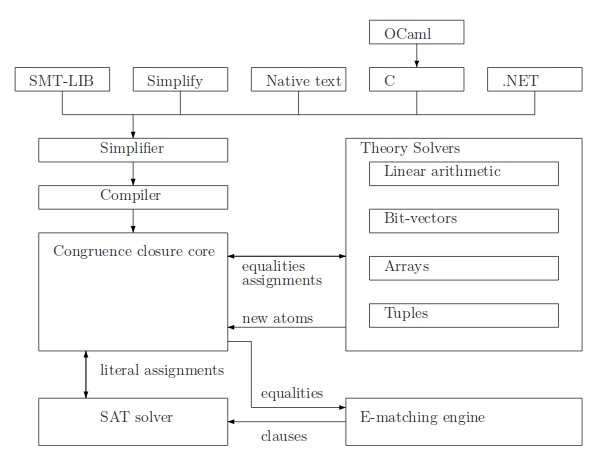
\includegraphics[width=1\textwidth]{arhitektura.png}
  \caption{Arhitektura rešavača Z3}
  \label{fig:arhitektura}
\end{figure}
\par
Formule prosleđene rešavaču se najpre procesiraju upotrebom simplifikacije. Simplifikacija primenjuje algebarska pravila redukcije kao što je \texttt{p $\land$ true $\vdash$ true}. Pored toga, ovim procesom se vrše odgovarajuće zamene kao što je \texttt{x=4 $\land$ q(x) $\vdash$ x=4 $\land$ q(4)}.
Nakon simplifikacije, kompajler formira apstraktno sintaksno stablo formula čiji su čvorovi simplifikovane formule (klauze). Zatim se jezgru kongruentnog zatvorenja (eng. 
\textit{Congruence closure core}) prosleđuje apstraktno sintaksno stablo. Jezgro kongruentnog zatvorenja komunicira sa SAT rešavačem koji određuje istinitosnu vrednost klauza. 
\par

Ulazni format rešavača Z3 je definisan SMT-LIB 2.0 standardom REF. Standard definiše jezik logičkih formula čija se zadovoljivost proverava u odnosu na neku teoriju. Verzija 2.0 imala je za cilj pojednostavljivanje jezika logičkih formula povecavanjem njihove izražajnosti i fleksibilnosti. Cilj standarda je obezbeđivanje zajedničkog jezika za sve SMT rešavače. 
\par
Interno, Z3 održava stek korisnički definisanih formula i deklaracija. Formule i deklaracije jednim imenom nazivamo tvrđenjima. Komandom \texttt{push} kreira se novi opseg i čuva se trenutna veličina steka. Komandom \texttt{pop} uklanjaju se sva tvrđenja i deklaracije zadate posle push-a sa kojim se komanda uparuje. Komandom \texttt{assert} dodaje se formula na interni stek. Skup formula na steku je zadovoljiv ako postoji interpretacija u kojoj sve formule imaju istinitosnu vrednost tačno. Ova provera se vrši komandom \texttt{check-sat}. U slučaju zadovoljivosti vraća se \texttt{sat}, u slučaju nezadovoljivosti vraća se \texttt{unsat} a kada rešavač ne može da proceni da li je formula zadovoljiva ili ne vraća se \texttt{unknown}. Komandom \texttt{get-model} vraća se interpretacija u kojoj su sve formule na steku tačne. 
\par
Glavni gradivni blokovi formula su konstante, funkcije i relacije. Konstante su specijalan slučaj funkcija bez parametara. Relacije su funkcije koje vraćaju povratnu vrednost tipa Boolean. Funkcije mogu uzimati argumente tipa Boolean pa se na taj način relacije mogu koristiti kao argumenti funkcija.  


Formula $F$ je validna ako je vrednost valuacije $true$ za bilo koje interpretacije funkcija i konstantnih simbola. Formula $F$ je zadovoljiva ukoliko postoji valuacija u kojoj je formula tačna. Da bismo odredili da li je formula $F$ validna, rešavač Z3 proverava da li je formula $\lnot F$ zadovoljiva. Ukoliko je negacija formule nezadovoljiva, onda je polazna formula validna. 

 

\section{Teorije} \label{sec:num2}
Teorije rešavača Z3 su opisane u okviru višesortne logike prvog reda sa jednakošću.  Definisanjem specifične teorije, uvode se restrikcije pri definisanju formula kao i podržanih relacija i operatora koje se nad njima primenjuju. Na taj način, specijalizovane metode u odgovarajućoj teoriji mogu biti efikasnije implementirane u poređenju sa opštim slučajem. U nastavku će biti opisane teorija neinterpretiranih funkcija, teorija linearne aritmetike, teorija nelinearne aritmetike, teorija bitvektora i teorija nizova.

\subsection{Teorija neinterpretiranih funkcija}
Teorije obično određuju interpretaciju funkcijskih simbola. Teorija koja ne zadaje nikakva ograničenja za funkcijske simbole naziva se teorija neinterpretiranih funkcija 
(eng. \textit{theory of equality with Uninterpreted Functions}, skraćeno EUF). Kod rešavača Z3, funkcije i konstantni simboli su neinterpretirani. Ovo je kontrast u odnosu na funkcije odgovarajućih teorija. Funkcija + ima standardnu interpretaciju u teoriji aritmetike. Neinterpretirane funkcije i konstante su maksimalno fleksibilne i dozvoljavaju bilo koju interpretaciju koja je u skladu sa ograničenjima. Za razliku od programskih jezika, funkcije logike prvog reda su totalne, tj. definisane su za sve vrednosti ulaznih parametara. Na primer, deljenje 0 je dozvoljeno, ali nije specifikovano šta ono predstavlja. Teorija neinterpretiranih funkcija je odlučiva i postoji procedura odlučivanja polinomijalne vremenske složenosti. Jedna od procedura odlučivanja za ovu teoriju zasniva se na primeni algoritma Nelson-Open (eng. \textit{Nelson-Open algorithm}). O ovom algoritmu može se više naći u literaturi. REFERENCA
\par

Komandom \texttt{declare-const} deklariše se konstanta odgovarajuće sorte (odgovara tipu promenljive u programskim jezicima). Sorta može biti parametrizovana i u tom slučaju su specifikovana imena njenih parametara. Specifikacija sorte vrši se naredbom \texttt{(define-sort [symbol] ([symbol]+)[sort])}.
Komandom \texttt{declare-fun} deklariše se funkcija. 
\begin{primer} Naredni kod demonstrira upotrebu konstanti i funkcija. U primeru se deklariše konstanta a celobrojnog tipa i funkcija f sa parametrima tipa Int i Bool i povratnom vrednošću tipa Int. Zatim se dodaju odgovarajuća ograničenja za konstantu a i funkciju f korišćenjem operatora poređenja. Rešavač Z3 pronalazi da je ovo tvrđenje zadovoljivo i daje prikazani model. 
\\ 

\hspace{-0.7cm}
\begin{minipage}[b]{0.43\textwidth}
\textbf{Formula prosleđena rešavaču:}\\
(declare-const a Int)\\
(declare-fun f (Int Bool) Int)\\
(assert (> a 10))\\
(assert (< (f a true) 100))\\
(check-sat)\\
(get-model) \\
\end{minipage}
\hspace{0.6cm}
\begin{minipage}[t]{0.5\textwidth}
\vspace{-4.715cm}
\textbf{Izlaz:}
\\sat 
\\(model 
\\\tab(define-fun a () Int 11) 
\\\tab(define-fun f ((x!1 Int) (x!2 Bool)) Int 
\\\tab(ite (and (= x!1 11) (= x!2 true)) 0 0))
\\)
\end{minipage}
\end{primer}

U narednom primeru koristimo pomenutu činjenicu da se validnost formule pokazuje ispitivanjem zadovoljivosti negirane formule. 

\begin{primer} Dokazivanje de Morganovog zakona dualnosti ispitivanjem validnosti formule: $\neg{(a \land b)} \Leftrightarrow (\neg{a} \lor \neg{b}) $ tako što se kao ograničenje dodaje negacija polazne formule. Z3 pronalazi da je negacija formule nezadovoljiva, pa je polazna formula tačna u svim interpretacijama. \\

\hspace{-0.6cm}
\begin{minipage}[b]{0.5\textwidth}
\textbf{Formula prosleđena rešavaču:}
\\(declare-const a Bool)
\\(declare-const b Bool)
\\(define-fun demorgan () Bool
\\\tab (= (and a b) (not (or (not a) (not b))))
\\)
\\(assert (not demorgan))
\\(check-sat) 
\\(get-model)
\end{minipage}
\hspace{1.5cm}
\begin{minipage}[t]{0.4\textwidth}
\vspace{-5.35cm}
\textbf{Izlaz:}
\\unsat
\end{minipage}
\end{primer}


\subsection{Teorija linearne aritmetike} 

Rešavač Z3 sadrži procedure odlučivanja za linearnu aritmetiku nad celobrojnim i realnim brojevima. Dodatni materijali o procedurama odlučivanja linearne aritmetike dostupni su u literaturi \cite{FastLinearArithmetic}.
\par

U okviru celobrojne linearne aritmetike, podržani funkcijski simboli su +, - i * gde je drugi operand konstanta. Nad funkcijskim simbolima, čiji su specijalni slučajevi konstante mogu se primenjivati relacijski operatori <, <=, > i >=. 
\par
U okviru realne linearne aritmetike, podržani funkcijski simboli su +, - i * pri čemu je drugi operand konstanta. Pored ovih podržane su operacije div i mod, uz uslov da je drugi operand konstanta različita od 0. Nad funkcijskim simbolima, čiji su specijalni slučajevi konstante mogu se primenjivati relacijski operatori <, <=, > i >=. 
\par
Rešavač Z3 ima podršku za celobrojne i realne konstante. Prethodno pomenutom komandom \texttt{declare-const} deklarišu se celobrojne i realne konstante. Rešavač ne vrši automatsku konverziju između celobrojnih i realnih konstanti. U tom slučaju koristi se funkcija \texttt{to-real} za konvertovanje celobrojnih u realne vrednosti.
Realne konstante treba da budu zapisane sa decimalnom tačkom.

\begin{primer} Naredni kod ilustruje pronalaženje interpretacija celobrojnih i realnih konstanti. Interpretacija se svodi na pridruživanje brojeva svakoj konstanti. Ograničenja sadrže pomenute aritmetičke operatore. Rešavač vraća zadovoljivost tvrđenja i dobijeni model prikazujemo u nastavku.\\ \\
\begin{minipage}[b]{0.47\textwidth}
\textbf{Formula prosleđena rešavaču:}
\\(declare-const a Int)
\\(declare-const b Int)
\\(declare-const c Int)
\\(declare-const d Real)
\\(declare-const e Real)
\\(assert (> e (+ (to\_real (+ a b)) 2.0)))
\\(assert (= d (+ (to\_real c) 0.5)))
\\(check-sat)
\\(get-model)
\end{minipage}
\hspace{1.6cm}
\begin{minipage}[t]{0.4\textwidth}
\vspace{-6cm}
\textbf{Izlaz:}
\\sat 
\\(model
\\\tab(define-fun b () Int 0) 
\\\tab(define-fun a () Int 1) 
\\\tab(define-fun e () Real 4.0) 
\\\tab(define-fun c () Int 0) 
\\\tab(define-fun d () Real (/ 1.0 
\\\tab 2.0))
\\)
\end{minipage}

\end{primer}


Takođe, postoji uslovni operator (if-then-else operator). Na primer,
izraz (ite (and (= x!1 11) (= x!2 false)) 21 0) ima vrednost 21 kada je promenljiva x!1 jednaka 11, a promenljiva x!2 ima vrednost False. U suprotnom, vraća se 0.

U slučaju deljenja, može se koristiti ite (if-then-else) operator i na taj način se može dodeliti interpretacija u slučaju deljenja nulom.
\par
Mogu se konstruisati novi operatori, korišćenjem \texttt{define-fun} konstruktora. Ovo je zapravo makro, pa će rešavač vršiti odgovarajuće zamene.
\begin{primer} Kod definiše operator deljenja tako da rezultat bude specifikovan i kada je delilac 0. Uvode se dve konstante realnog tipa i primenjuje se definisani operator. Z3 rešavač pronalazi nezadovoljivost tvrđenja s obzirom da operator mydiv vraća 0 pa relacija poređenja ne može biti tačna.\\ \\
\begin{minipage}[b]{0.5\textwidth}
\textbf{Formula prosleđena rešavaču:}
\\(define-fun mydiv ((x Real) (y Real)) Real
\\\tab (if (not (= y 0.0))  (/ x y)  0.0))
\\(declare-const a Real)
\\(declare-const b Real)
\\(assert (>= (mydiv a b) 1.0))
\\(assert (= b 0.0))
\\(check-sat)
\end{minipage}
\hspace{3cm}
\begin{minipage}[t]{0.4\textwidth}
\vspace{-4.73cm}
\textbf{Izlaz:}
\\unsat
\end{minipage}
\end{primer}
\subsection{Teorija nelinearne aritmetike} 

Formula predstavlja formulu nelinearne aritmetike ako je oblika (* t s), pri čemu t i s nisu linearnog oblika.
Nelinearna celobrojna aritmetika je neodlučiva, tj. ne postoji procedura koja za proizvoljan ulaz vraća odgovor \texttt{sat} ili \texttt{unsat}. U najvećem broju slučajeva, Z3 vraća kao rezultat \texttt{unknown}. Postoje nelinearni problemi za koje Z3 rešavač vraća odgovarajući model koristeći procedure odlučivanja zasnovana na Grebnerovim bazama.

\begin{primer} Naredni primer ilustruje rešavanje različitih nelinearnih problema sa celobrojnim i realnim konstantama. Z3 rešavač ne pronalazi uvek model za nelinearne probleme, ovde se za drugo tvrđenje vraća nezadovoljivost. Kada su prisutna samo nelinearna ograničenja nad realnim konstantama, Z3 koristi posebne metode odlučivanja. Ove metode korišćene su za dokazivanje trećeg tvrđenja.\\ \\
\begin{minipage}[b]{0.43\textwidth}
\textbf{Formula prosleđena rešavaču:}
\\(declare-const a Int)
\\(assert (> (* a a) 3))
\\(check-sat)
\\(get-model)
\\(declare-const b Real)
\\(declare-const c Real)
\\(assert (= (+ (* b b b) (* b c)) 3.0))
\\(check-sat)
\\(declare-const b Real)
\\(declare-const c Real)
\\(assert (= (+ (* b b b) (* b c)) 3.0))
\\(check-sat)
\\(get-model)

\end{minipage}
\hspace{1cm}
\begin{minipage}[t]{0.45\textwidth}
\vspace{-8.5cm}
\textbf{Izlaz:}
\\sat 
\\(model 
\\\tab(define-fun a () Int (- 8))
\\) 
\\
\\unsat 
\\
\\sat 
\\(model 
\\\tab(define-fun b () Real (/ 1.0 8.0)) 
\\\tab(define-fun c () Real (/ 15.0 64.0))
\\)
\end{minipage}
\end{primer}

\subsection{Teorija bitvektora} 
Rešavač Z3 podržava vektore proizvoljne dužine. \texttt{(\_ BitVec n)} je sorta bitvektora čija je dužina \texttt{n}. Bitvektor literali se mogu definisati koristeći binarnu, decimalnu ili heksadecimalnu notaciju. U binarnom i heksadecimalnom slučaju, veličina bitvektora je određena brojem karaktera. Na primer, literal \textit{\#b010} u binarnom formatu je bitvektor dužine 3, a literal \textit{\#x0a0} u heksadecimalnom formatu je bitvektor veličine 12. Veličina bitvektora mora biti specifikovana u decimalnom formatu. Na primer, reprezentacija \textit{(\_ bv10 32)} je bitvektor dužine 32 sa vrednošću 10. Podrazumevano, Z3 predstavlja bitvektore u heksadecimalnom formatu ukoliko je dužina bitvektora umnožak broja 4 a u suprotnom u binarnom formatu. Komanda 
\texttt{(set-option :pp.bv-literals false)} se može koristiti za predstavljanje literala bitvektora u decimalnom formatu. Više materijala o procedurama odlučivanja za teoriju bitvektora može se naći u literaturi \cite{DPBitvector}.
\begin{primer} Navodimo različite načine predstavljanja bitvektora. Ukoliko zapis počinje sa \#b, bitvektor se zapisuje u binarnom formatu. Ukoliko zapis počinje sa \#x, bitvektor se zapisuje u heksadecimalnom formatu. U oba slučaja, nakon specifikacije formata, zapisuje se dužina vektora. Drugi način zapisa počinje skraćenicom bv, navođenjem vrednosti i na kraju dužine. Komandom \texttt{(display t)} štampa se izraz \texttt{t}.\\\\
\begin{minipage}[b]{0.45\textwidth}
\textbf{Formula prosleđena rešavaču:}
\\(display \#b0100)
\\(display (\_ bv20 8))
\\(display (\_ bv20 7))
\\(display \#x0a) 
\\(set-option :pp.bv-literals false)
\\(display \#b0100)
\\(display (\_ bv20 8))
\\(display (\_ bv20 7))
\\(display \#x0a)
\end{minipage}
\hspace{2.5cm}
\begin{minipage}[t]{0.4\textwidth}
\vspace{-5.93cm}
\textbf{Izlaz:}
\\\#x4 
\\\#x14 
\\\#b0010100 
\\\#x0a 
\\(\_ bv4 4) 
\\(\_ bv20 8) 
\\(\_ bv20 7) 
\\(\_ bv10 8)
\end{minipage}
\end{primer}

Pri korišćenju operatora nad bitvektorima, mora se eksplicitno navesti tip operatora. Zapravo, za svaki operator podržane su dve varijante za rad sa označenenim i neoznačenim operandima. Ovo je kontrast u odnosu na programske jezike u kojima kompajler na osnovu argumenata implicitno određuje tip operacije (označena ili neoznačena varijanta).
\par
U skladu sa prethodno navedenom činjenicom, teorija bitvektora ima na raspolaganju različite verzije aritmetičkih operacija za označene i neoznačene operande. Za rad sa bitvektorima od aritmetičkih operacija definisane su operacije sabiranja, oduzimanja, određivanje negacije (zapisivanja broja u komplementu invertovanjem svih bitova polaznog broja), množenja, izračunavanja modula pri deljenju, šiftovanje u levo kao i označeno i neoznačeno šifrovanje u desno. Podržane su sledeće logičke operacije: disjunkcija, konjunkcija, unarna negacija, negacija konjunkcije i negacija disjunkcije. Definisane su različite relacije nad bitvektorima kao što su <=, <, >=, >.

\begin{primer} Naredni primer ilustruje aritmetičke operacije nad bitvektorima. Podržane aritmetičke operacije su sabiranje (bvadd), oduzimanje (bvsub), unarna negacija (bvneg), množenje (bvmul), računanje modula (bvmod), šiftovanje ulevo (bvshl), neoznačeno (logičko) šiftovanje udesno (bvlshr) i označeno (aritmetičko) šiftovanje udesno (bvashr). Od logičkih operacija postoji podrška za disjunkciju (bvor), konjunkciju (bvand), ekskluzivnu disjunkciju (bvxor), negaciju disjunkcije (bvnor), negaciju konjunkcije (bvnand) i negaciju ekskluzivne disjunkcije (bvnxor).
Komandom \texttt{(simplify t)} prikazuje se jednostavniji izraz ekvivalentan izrazu \texttt{t} ukoliko postoji.
\\\\
\begin{minipage}[b]{0.5\textwidth}
\textbf{Formula prosleđena rešavaču:}
\\(simplify (bvadd \#x07 \#x03)) 
\\(simplify (bvsub \#x07 \#x03)) 
\\(simplify (bvneg \#x07))       
\\(simplify (bvmul \#x07 \#x03)) 
\\(simplify (bvsmod \#x07 \#x03)) 
\\(simplify (bvshl \#x07 \#x03)) 
\\(simplify (bvlshr \#xf0 \#x03))  
\\(simplify (bvashr \#xf0 \#x03))  
\\(simplify (bvor \#x6 \#x3)) 
\\(simplify (bvand \#x6 \#x3))  
\\(simplify (bvxor \#x6)) 
\\(simplify (bvnand \#x6 \#x3)) 
\\(simplify (bvnor \#x6 \#x3)) 
\\(simplify (bvxnor \#x6 \#x3)) 
\end{minipage}
\hspace{2.5cm}
\begin{minipage}[b]{0.5\textwidth}
\textbf{Izlaz:}
\\\#x0a 
\\\#x04 
\\\#xf9 
\\\#x15 
\\\#x01 
\\\#x38 
\\\#x1e 
\\\#xfe
\\\#x7 
\\\#x2 
\\\#x9 
\\\#xd 
\\\#x8 
\\\#xa
\end{minipage}

\end{primer}


\par
\begin{primer} 
Postoji brz način da se proveri da li su brojevi fiksne dužine stepeni dvojke. 
Ispostavlja se da je bitvektor x stepen dvojke ako i samo ako je vrednost izraza x $\land$ (x - 1) jednaka 0. Dodaje se negacija ove jednakosti kao tvrđenja i vrši se proveravanje za bitvektore vrednosti 0, 1, 2, 4 i 8. U svim slučajevima brojevi su stepeni dvojke pa Z3 rešavač vraća nezadovoljivost.\\ \\
\begin{minipage}[b]{0.5\textwidth}
\textbf{Formula prosleđena rešavaču:}
\\(define-fun is-power-of-two 
\\\tab((x (\_ BitVec 4))) Bool 
\\\tab(= \#x0 (bvand x (bvsub x \#x1)))
\\)
\\(declare-const a (\_ BitVec 4))
\\(assert 
\\\tab(not (= (is-power-of-two a) 
\\\tab\tab    (or (= a \#x0) 
\\\tab\tab\tab     (= a \#x1) 
\\\tab\tab\tab     (= a \#x2) 
\\\tab\tab\tab     (= a \#x4) 
\\\tab\tab\tab     (= a \#x8)
\\\tab\tab		))
\\\tab )
\\)
\\(check-sat)
\end{minipage}
\hspace{2.5cm}
\begin{minipage}[t]{0.5\textwidth}
\vspace{-10.45cm}
\textbf{Izlaz:}
\\unsat
\end{minipage}
\end{primer}

\begin{primer} Primer ilustruje upotrebu relacija nad bitvektorima. Podržane relacije uključuju neoznačene i označene verzije za operatore <, <=, > i >=. Neoznačene varijante počinju nazivom bvu, a u nastavku sledi ime relacije. Na primer, relacija <= nad neoznačenim brojevima zadaje se komandom bvule, a relacija > nad neoznačenim brojevima komandom bvugt. Označene varijante počinju nazivom bvs, a u nastavku ponovo sledi ime relacije. Na primer, relacija >= nad neoznačenim brojevima zadaje se komandom bvsge, a relacija < nad označenim brojevima komandom bvslt.
\\ \\ 
\begin{minipage}[b]{0.5\textwidth}
\textbf{Formula prosleđena rešavaču:}
\\(simplify (bvule \#x0a \#xf0))  
\\(simplify (bvult \#x0a \#xf0))  
\\(simplify (bvuge \#x0a \#xf0))  
\\(simplify (bvugt \#x0a \#xf0))  
\\(simplify (bvsle \#x0a \#xf0)) 
\\(simplify (bvslt \#x0a \#xf0))  
\\(simplify (bvsge \#x0a \#xf0))  
\\(simplify (bvsgt \#x0a \#xf0))

\end{minipage}
\hspace{2cm} 
\begin{minipage}[t]{0.5\textwidth}
\vspace{-5.3cm}
\textbf{Izlaz:}
\\true 
\\true 
\\false 
\\false 
\\false 
\\false 
\\true 
\\true
\end{minipage}


\end{primer}

Rešavač Z3 nudi funkcije za promenu načina reprezentacije brojeva. Moguće su konverzije reprezentacije brojeva linearne aritmetike u reprezentaciju bitvektora i obrnuto. Ovaj rezultat može se postići naredbama: \\
\texttt{(define b (int2bv[32] z))} \\  
\texttt{(define c (bv2int[Int] x))} 
\begin{primer} Primer poredi bitvektore koristeći označene i neoznačene verzije operatora. Označeno poređenje, kao što je bvsle, uzima u obzir znak bitvektora za poređenje, dok neoznačeno poređenje tretira bitvektor kao prirodan broj. Z3 rešavač pronalazi da je tvrđenje zadovoljivo i daje prikazani model.
\\ \\
\begin{minipage}[b]{0.5\textwidth}
\textbf{Formula prosleđena rešavaču:}
\\(declare-const a (\_ BitVec 4))
\\(declare-const b (\_ BitVec 4))
\\(assert (not (= (bvule a b) (bvsle a b)))
\\(check-sat)
\\(get-model)
\end{minipage}
\hspace{1.15cm} 
\begin{minipage}[t]{0.5\textwidth}
\vspace{-3.45cm}
\textbf{Izlaz:}
\\sat 
\\(model 
\\\tab(define-fun b () (\_ BitVec 4) \#xe) 
\\\tab(define-fun a () (\_ BitVec 4) \#x0)
\\)
\end{minipage}


\end{primer}


\subsection{Teorija nizova} 
Osnovnu teoriju nizova karakterišu \texttt{select} i \texttt{store} naredbe. 
Komandom \texttt{(select a i)} vraća se vrednost na poziciji i u nizu a, a izraz \texttt{(store a i v)} formira novi niz, identičan nizu a pri čemu se na poziciji i nalazi vrednost v.
Z3 sadrži procedure odlučivanja za osnovnu teoriju nizova.
Dva niza su jednaka ukoliko su vrednosti svih elemenata na odgovarajućim pozicijama jednake.
 
\begin{primer} Definišemo tri konstante x, y i z celobrojnog tipa. Neka je a1 niz celobrojnih vrednosti. Tada je ograničenje (and (= (select a1 x) x) (= (store a1 x y) a1)) zadovoljivo kada je element niza a na poziciji x jednak definisanoj konstanti x i u slučaju kada su konstante x i y jednake.
Rešavač Z3 vraća zadovoljivost zadatog tvrđenja i odgovarajući model.
 \\ \\
\begin{minipage}[b]{0.45\textwidth}
\textbf{Formula prosleđena rešavaču:}
\\(declare-const x Int)
\\(declare-const y Int)
\\(declare-const z Int)
\\(declare-const a1 (Array Int Int))
\\(assert (= (select a1 x) x))
\\(assert (= (store a1 x y) a1))
\\(check-sat)
\\(get-model)
\end{minipage}
\hspace{1.3cm} 
\begin{minipage}[t]{0.5\textwidth}
\vspace{-5.3cm}
\textbf{Izlaz:}
\\sat
\\(model 
\\\tab(define-fun y () Int 1)
\\\tab(define-fun a1 () (Array Int Int)
\\\tab\tab(\_ as-array k!0)
\\\tab)
\\\tab(define-fun x () Int 1)
\\\tab(define-fun k!0 
\\\tab\tab((x!1 Int)) Int (ite (= x!1 1) 1 0)
\\\tab)
\\)
\end{minipage}
\end{primer} 
 

\subsubsection{Konstantni nizovi}

Nizovi sa konstantnim vrednostima mogu se specifikovati koristeći \texttt{const} konstrukciju. Upotrebom const konstrukcije Z3 ne može da odluči kog tipa su elementi niza pa se on mora eksplicitno navesti. Interpretacija nizova je slična interpretaciji funkcija. Z3 koristi konstrukciju \texttt{(\_ as-array f)} za određivanje interpretacije niza. Ako je niz a jednak rezultatu konstrukcije \texttt{(\_ as-array f)}, tada za svaki indeks i, vrednost \texttt{(select a i)} odgovara vrednosti \texttt{(f i)}. 

\begin{primer} Definišemo konstantni niz m celobrojnog tipa i dve celobrojne konstante a i i. Uvodimo ograničenje da niz m sadrži samo jedinice. Z3 pronalazi da je ovo tvrdjenje zadovoljivo, i daje prikazani model.\\
\begin{minipage}[b]{0.55\textwidth}
\vspace{0.5cm} 
\textbf{Formula prosleđena rešavaču:}
\\(declare-const m (Array Int Int))
\\(declare-const a Int)
\\(declare-const i Int)
\\(assert (= m ((as const (Array Int Int)) 1)))
\\(assert (= a (select m i)))
\\(check-sat)
\\(get-model)
\end{minipage}
\hspace{1.1cm} 
\begin{minipage}[t]{0.5\textwidth}
\vspace{-4.7cm}
\textbf{Izlaz:}
\\sat 
\\(model 
\\\tab(define-fun m () (Array Int Int) 
\\\tab\tab(\_ as-array k!0)
\\\tab) 
\\\tab(define-fun i () Int 0) 
\\\tab(define-fun a () Int 1) 
\\\tab(define-fun k!0 ((x!0 Int)) 
\\\tab\tab Int (ite (= x!0 0) 1 1)
\\\tab)
\\)
\end{minipage}
\end{primer}

\subsubsection{Primena map funkcije na nizove}
Rešavač Z3 obezbeđuje primenu parametrizovane funkcije map na nizove. Funkcijom map omogućava se primena proizvoljnih funkcija na sve elemente niza.
\begin{primer} Definišemo dva konstantna niza a i b tipa Boolean i dokazujemo da važi svojstvo $\neg{(a \land b)} \Leftrightarrow (\neg{a} \lor \neg{b}) $ primenom funkcije map na sve elemente nizova. Kao ograničenje dodajemo negaciju prethodno navedene formule. Rešavač Z3 vraća nezadovoljivost negirane formule, odakle zaključujemo da je polazna formula validna.\\ \\
\begin{minipage}[b]{0.65\textwidth}
\textbf{Formula prosleđena rešavaču:}
\\(define-sort Set (T) (Array T Bool))
\\(declare-const a (Set Int))
\\(declare-const b (Set Int))
\\(assert (not (= ((\_ map and) a b) ((\_ map not) 
\\\tab((\_ map or) ((\_ map not) b) ((\_ map not) a)))))
\\)
\\(check-sat)
\end{minipage}
\hspace{2.5cm} 
\begin{minipage}[t]{0.5\textwidth}
\vspace{-4.65cm}
\textbf{Izlaz:}
\\unsat 
\end{minipage}
\end{primer}

Nad nizovima se mogu vršiti slične operacije kao i nad skupovima. Rešavač Z3 ima podršku za računanje unije, preseka i razlike dva niza. Ovi operatori se tumače na isti način kao i u teoriji skupova. Za nizove a i b, pomenuti operatori mogu se koristiti navođenjem komandi:\\
\texttt{(union a b)} ; kreiranje unije dva niza kao skupa \\
\texttt{(intersect a b)} ; kreiranje preseka dva niza kao skupa \\
\texttt{(difference a b)} ; kreiranje razlike dva niza kao skupa
\section{Tipovi podataka} \label{sec:num3}

Algebarski tipovi podataka omogućavaju specifikaciju uobičajnih struktura podataka. Slogovi, torke i skalari (enumeracijski tipovi) spadaju u algebarske tipove podataka. Primena algebarskih tipova podataka može se generalizovati. Mogu se koristiti za specifikovanje konačnih listi, stabala i rekurzivnih struktura. 
\subsection{Slogovi}
Slog se specifikuje kao tip podataka sa jednim konstruktorom i proizvoljnim brojem elemenata sloga. Rešavač Z3 ne dozvoljava povećavanje broja argumenata sloga nakon njegovog definisanja. Važi svojstvo da su dva sloga jednaka samo ako su im svi argumenti jednaki.

\begin{primer} Pokazujemo svojstvo da su dva sloga jednaka ako i samo ako su im svi argumenti jednaki. Uvodimo parametarski tip Pair, sa konstruktorom mk-pair i dva argumenta kojima se može pristupiti koristeći selektorske funkcije first i second. Definišemo dva sloga p1 i p2, čija su oba podatka celobrojnog tipa. Dodajemo ograničenja da su slogovi p1 i p2 jednaki kao i ograničenje koje se odnosi na drugi element sloga. Rešavač Z3 u prvom slučaju vraća zadovoljivost formule i odgovarajući model. Dodavanjem ograničenja da prvi elementi slogova nisu jednaki korišćenjem selektorske funkcije first, tvrđenje postaje nezadovoljivo.
\\ \\
\begin{minipage}[b]{0.5\textwidth}
\textbf{Formula prosleđena rešavaču:}
\\(declare-datatypes (T1 T2) 
\\\tab[0.3cm](Pair (mk-pair (first T1) (second T2))))
\\(declare-const p1 (Pair Int Int))
\\(declare-const p2 (Pair Int Int))
\\(assert (= p1 p2))
\\(assert (> (second p1) 20))
\\(check-sat)
\\(get-model)
\\(assert (not (= (first p1) (first p2))))
\\(check-sat)
\end{minipage}
\hspace{1.5cm} 
\begin{minipage}[t]{0.5\textwidth}
\vspace{-6.59cm}
\textbf{Izlaz:}
\\sat 
\\(model 
\\\tab(define-fun p1 () (Pair Int Int) 
\\\tab\tab(mk-pair 0 21)
\\\tab) 
\\\tab(define-fun p2 () (Pair Int Int) 
\\\tab\tab(mk-pair 0 21)
\\\tab)
\\unsat
\end{minipage}

\end{primer}
\subsection{Skalari (tipovi enumeracije)}

Sorta skalara je sorta konačnog domena. Elementi konačnog domena se tretiraju kao različite konstante. Na primer, neka je S skalarni tip sa tri vrednosti A, B i C. Moguće je da tri konstante skalarnog tipa S budu različite. Ovo svojstvo ne može važiti u slučaju četiri konstante.

\begin{primer} Prilikom deklaracije skalarnog tipa podataka, navodi se broj različitih elemenata domena, u ovom primeru tri i pokazuje se nezadovoljivost tvrđenja sa četiri različita elementa domena. \\ \\
\begin{minipage}[b]{0.5\textwidth}
\textbf{Formula prosleđena rešavaču:}
\\(declare-datatypes () ((S A B C)))
\\(declare-const x S)
\\(declare-const y S)
\\(declare-const z S)
\\(declare-const u S)
\\(assert (distinct x y z))
\\(check-sat)
\\(get-model)
\\(assert (distinct x y z u))
\\(check-sat)
\end{minipage}
\hspace{2.5cm} 
\begin{minipage}[t]{0.5\textwidth}
\vspace{-6.58cm}
\textbf{Izlaz:}
\\sat 
\\(model 
\\\tab(define-fun z () S A) 
\\\tab(define-fun y () S B) 
\\\tab(define-fun x () S C)  
\\)
\\unsat
\end{minipage}
\end{primer}

\subsection{Rekurzivni tipovi podataka}

Deklaracija rekurzivnog tipa podataka uključuje sebe direktno kao komponentu. Standardni primer rekurzivnog tipa podataka je lista. 
Lista celobrojnih vrednosti sa imenom \texttt{list} može se deklarisati naredbom:\\
\texttt{(declare-datatypes ((list (nil) (cons (hd Int) (tl list))))}
\par
Rešavaš Z3 ima ugrađenu podršku za liste korišćenjem ključne reči \texttt{List}.
Prazna lista se definiše korišćenjem klučne reči \texttt{nil} a konstruktor \texttt{insert} se koristi za dodavanje elemenata u listu. Selektori \texttt{head} i \texttt{tail} se definišu na uobičajan način.

\begin{primer} Deklarišemo tri liste l1, l2 i l3 sa celobrojnim vrednostima, kao i celobrojnu konstantu x. Dodaju se ograničenja za prve elemente listi l1 i l2 korišćenjem selektora. Pored toga, dodaje se ograničenje da liste l1 i l2 nisu jednake, tj. da nisu svi elementi na odgovarajućim pozicijama u listama jednaki. U listu l2 dodaje se konstanta x. Rešavač Z3 vraća zadovoljivost tvrđenja i dobrijeni model prikazujemo u nastavku.
\\ \\
\begin{minipage}[b]{0.42\textwidth}
\textbf{Formula prosleđena rešavaču:}
\\(declare-const l1 (List Int))
\\(declare-const l2 (List Int))
\\(declare-const l3 (List Int))
\\(declare-const x Int)
\\(assert (not (= l1 nil)))
\\(assert (not (= l2 nil)))
\\(assert (= (head l1) (head l2)))
\\(assert (not (= l1 l2)))
\\(assert (= l3 (insert x l2)))
\\(assert (> x 100))
\\(check-sat)
\\(get-model)
\end{minipage}
\hspace{0.9cm}
\begin{minipage}[t]{0.55\textwidth}
\vspace{-7.84cm}
\textbf{Izlaz:}
\\sat 
\\(model 
\\\tab(define-fun l3 () (List Int) 
\\\tab(insert 101 (insert 0 (insert 1 nil)))
\\\tab(define-fun x () Int 101) 
\\\tab(define-fun l1 () (List Int) (insert 0 nil)) 
\\\tab(define-fun l2 () (List Int) (insert 0 
\\\tab\tab(insert 1 nil))
\\\tab)
\\) 
\end{minipage}


\end{primer}

U prethodnom primeru, uvode se ograničenja da su liste l1 i l2 različite od nil. Vrši se uvođenje ovih ograničenja jer interpretacija selektora head i tail 
nije specifikovana u slučaju praznih lista.


\section{Interfejsi rešavača}  \label{sec:num4}
Rešavač Z3 obezbeđuje interfejse za direktnu podršku sa programskim jezicima C, C++ i Python. U nastavku će biti navedeni primeri korišćenja C++ API-ja za komunikaciju sa rešavačem Z3.

\begin{primer} Primer demonstrira upotrebu neinterpretiranih funkcija dokazivanjem formule x = y => g(x) = g(y), pri čemu su x i y celobrojne konstante, a g funkcijski simbol arnosti 1. Najpre se deklariše kontekst koji se prosleđuje rešavaču, a zatim celobrojne konstante x i y. Nakon toga, deklariše se funkcijski simbol g, sa ulaznim parametrom celobrojne sorte i izlaznom vrednošću celobrojne sorte. Dodaje se negacija prethodno navedene formule. U zavisnosti od rezultata, štampa se odgovarajuća poruka.\\
\begin{lstlisting}[language=C++]
void primer_sa_neinterpretiranim_funkcijama() { 
    context c;
    expr x      = c.int_const("x");
    expr y      = c.int_const("y");
    sort I      = c.int_sort();
    func_decl g = function("g", I, I);
    
    solver s(c);
    expr e = implies(x == y, g(x) == g(y));
    s.add(!e);
    if (s.check() == unsat) 
        std::cout << "dokazano";
    else
        std::cout << "nije dokazano";
}
\end{lstlisting}
\end{primer}\par
U slučaju zadovoljivosti tvrđenja, interpretacije konstanti modela mogu se koristiti za dalja izračunavanja.
\begin{primer} Primer demonstrira evaluaciju izraza u modelu. Najpre se definiše kontekst c i celobrojne konstante x i y. Zatim se rešavaču prosleđuju ograničenja x < y i x > 2. Proverava se zadovoljivost ograničenja i traži model. Na kraju se vrši evaluacija izraza x+y. 
\begin{lstlisting}[language=C++]
void eval_primer() {
    context c;
    expr x = c.int_const("x");
    expr y = c.int_const("y");
    solver s(c);

    s.add(x < y);
    s.add(x > 2);
    std::cout << s.check() << "\n";
    
    model m = s.get_model();
    std::cout << "Model:" << m;
    std::cout << "x+y = " << m.eval(x+y);
}
\end{lstlisting}
\end{primer}\par
U nastavku sledi dokazivanje validnosti formule pokazivanjem nezadovoljivosti njene negacije.
\begin{primer} Primer demonstrira dokazivanje De Morganovog zakona korišćenjem C++ API-ja i ranije pomenute formule. Na početku se deklariše kontekst, konstante x i y kao i izraz e čija se validnost ispituje. Rešavaču se prosleđuje negacija izraza kao ograničenje i ispituje se zadovoljivost negirane formule. U zavisnosti od rezultata štampa se odgovarajuća poruka.
\begin{lstlisting}[language=C++]
void demorgan() {
    context c;
    expr x = c.bool_const("x");
    expr y = c.bool_const("y");
    expr e = (!(x && y)) == (!x || !y);
    
    solver s(c);
    s.add(!e);

    switch (s.check()) {
    case unsat:   std::cout << "Formula je validna"; break;
    case sat:     std::cout << "Formula nije validna"; break;
    case unknown: std::cout << "Rezultat je nepoznat"; break;
    }
}
\end{lstlisting}
\end{primer}

U nastavku sledi problem pronalaženja modela u linearnoj aritmetici korišćenjem C++ API-ja. 
\begin{primer} Primer ilustruje traženje interpretacija celobrojnih konstanti x i y, pri čemu moraju biti ispunjene nejednakosti x >= 1 i y < x+3. Na početku se deklariše kontekst c i celobrojne konstante x i y. Zatim se rešavaču prosleđuju ograničenja i traži model. U okviru modela, pronalaze se interpretacije funkcijskih simbola. U ovom slučaju to su interpretacije konstanti, kao funkcijskih simbola arnosti 0. Na kraju se za svaku od konstanti ispisuje njeno ime i dodeljena vrednost. \\
\begin{lstlisting}[language=C++]
void primer_linearne_aritmetike() {
    context c;
    expr x = c.int_const("x");
    expr y = c.int_const("y");
    solver s(c);
    s.add(x >= 1);
    s.add(y < x + 3);
    model m = s.get_model();

    for(unsigned i = 0; i < m.size(); i++) {
        func_decl v = m[i];
        assert(v.arity() == 0); 
        std::cout << v.name() << "=" << m.get_const_interp(v);
    }
}
\end{lstlisting}
\end{primer}


U nastavku sledi problem pronalaženja modela u nelinearnoj aritmetici korišćenjem C++ API-ja. 
\begin{primer}
Primer ilustruje traženje interpretacija realnih konstanti x, y i z, pri čemu moraju biti ispunjene nejednakosti \(x^2 + y^2 = 1\) i \(x^3 + z^3 < 1/2\). Najpre se definiše kontekst i realne konstante x, y, z a zatim se rešavaču prosleđuju pomenuta ograničenja. Rešavač pronalazi interpretaciju realnih konstanti koje se zapisuju najpre u celobrojnom formatu, a zatim i u realnom formatu.
\\
\begin{lstlisting}[language=C++]
void primer_nelinearne_aritmetike() {    
    context c;
    expr x = c.real_const("x");
    expr y = c.real_const("y");
    expr z = c.real_const("z");
                     
    solver s(c);
    s.add(x*x + y*y == 1);                    
    s.add(x*x*x + z*z*z < c.real_val("1/2"));  
    
    std::cout << s.check();
    model m = s.get_model();
    std::cout << m << "\n";
    c.set(":pp-decimal", true); 
    std::cout << m;
}
\end{lstlisting}
\end{primer}

U nastavku sledi upotreba bitvektora korišćenjem C++ API-ja za komunikaciju za Z3 rešavačem.
\begin{primer} Primer pronalazi interpretacije konstanti x i y koje imaju reprezentaciju bitvektora. Deklariše se kontekst c i dve konstante x i y predstavljene bitvektorima dužine 32. Dodaje se ograničenje \(x^y - 103 = x*y\). Rešavač vraća zadovoljivost prosleđenih ograničenja a u nastavku se ispisuju imena i vrednosti konstanti.
\begin{lstlisting}[language=C++]
void primer_sa_bitvektorima() {
    context c;
    expr x = c.bv_const("x", 32);
    expr y = c.bv_const("y", 32);

    solver s(c);
    s.add((x ^ y) - 103 == x * y);
    std::cout << s.check();
    std::cout << s.get_model();
    
    for(unsigned i = 0; i < m.size(); i++) {
        func_decl v = m[i];
        assert(v.arity() == 0); 
        std::cout << v.name() << "=" << m.get_const_interp(v);
    }
}

\end{lstlisting}
\end{primer}

------------------------------------------------------------------------------

% ------------------------------------------------------------------------------
\chapter{Zaključak}
% ------------------------------------------------------------------------------


% ------------------------------------------------------------------------------
% Literatura
% ------------------------------------------------------------------------------
\literatura

% ==============================================================================
% Završni deo teze i prilozi
\backmatter
% ==============================================================================

% ------------------------------------------------------------------------------
% Biografija kandidata
\begin{biografija}
  
\end{biografija}
% ------------------------------------------------------------------------------

\end{document}
